\clearpage
\chapter{Results}

\section{Result exhaustive search}
    
    \subsection{Training}
        In figure \ref{training_overveiw_fig} an example plot in illustrated of how I monitored the training process. This example is too small for you to see any details, and so I will describe the most important details more closely. The example comes from the final logging of the model trained on all frequencies.
        \clearpage
        \begin{figure}[H]
            \centering
            \includegraphics[scale=0.3]{figures/epoch_50_test_38kHz_18kHz_70kHz_120kHz_200kHz_333kHz.png}
            \caption[Training example monitoring]{Example training monitoring. The upper row shows the network's output for each class on a validation sample, with and without a threshold applied. In the lower row, the labels for each, with the historical loss and F1-score plots. Yellow is values close to 1 and purple is 0.}
          	\medskip 
            \label{training_overveiw_fig}
        \end{figure}
        
        
        Extracted from figure \ref{training_overveiw_fig} figure illustrates
        \ref{loss_f1_duo_plot_fig} both validation and the training follows the same values and convergence trend. The F1-score for validation and training data follows the same approximately same values, showing no issues regarding over-/under-fitting. Finally, the sanity check visualize good performance on correctly identifying \textit{sandeel} class as illustrated in figure \ref{sandeel_threshold_label}.%(add more examples to appendix?) 
        
        \clearpage
        \begin{figure}[H]
            \centering
            \subfloat[\centering Loss]{{\includegraphics[width=5cm]{figures/Loss_val_train.png} }}%
            \qquad
            \subfloat[\centering F1-score]{{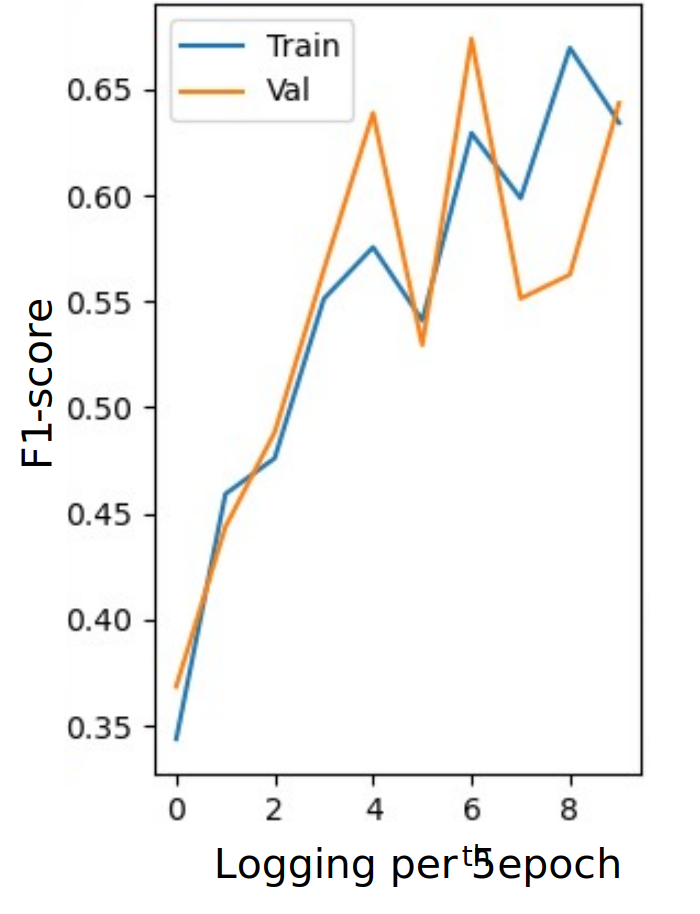
\includegraphics[width=5cm]{figures/F1_score_per_5.png} }}%
            \caption[Loss and F1 score during training]{The F1-score and loss for both training and validation. The validation loss was calculated less often, resulting in larger steps. The training and validation F1-score on the final validation data was respectively 0.63 and 0.64}%
            \label{loss_f1_duo_plot_fig}%
        \end{figure}
            
        \begin{figure}[H]
            \centering
            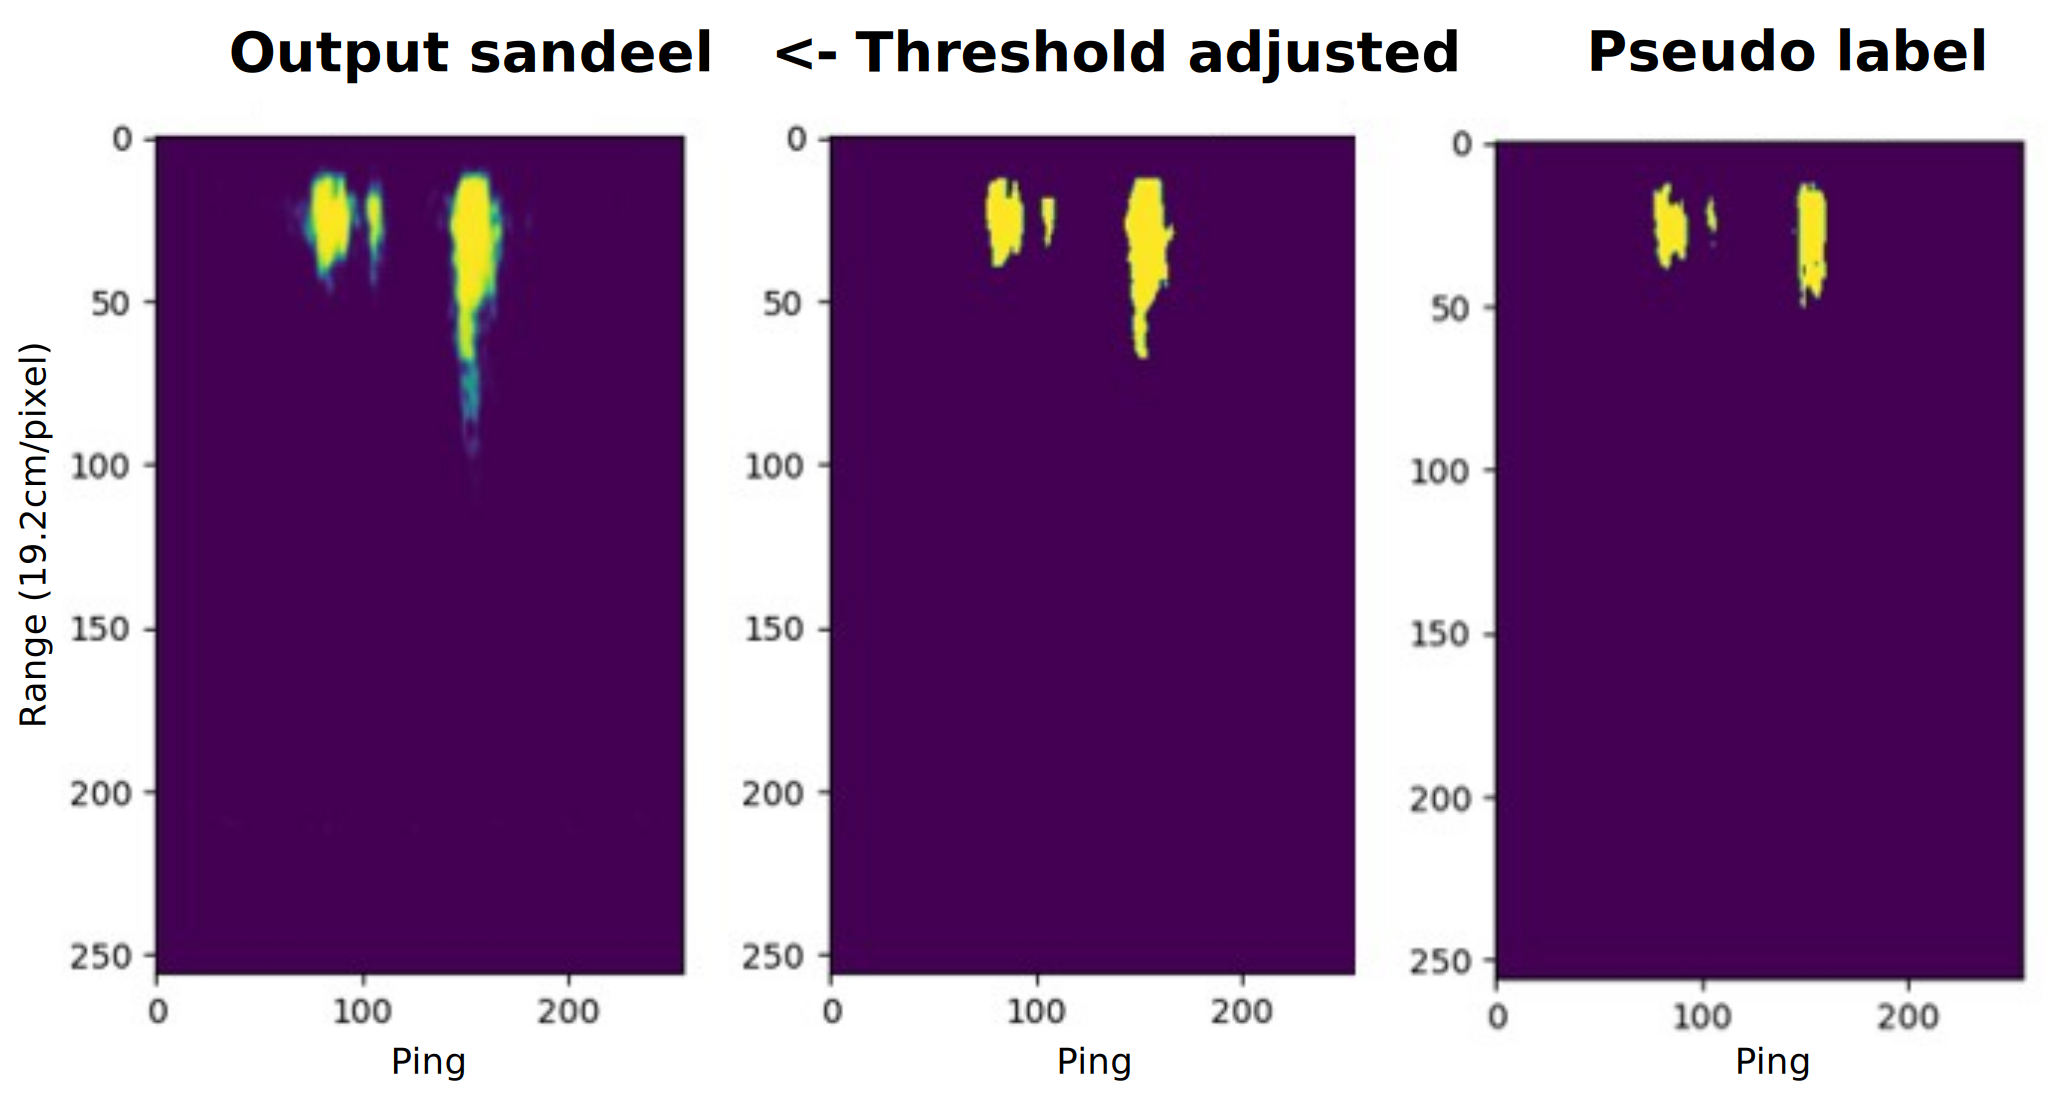
\includegraphics[scale=0.6]{figures/SANDEEL_WITH_LABEL.png}
            \caption[Examle output, threshold and label]{From left to right; Network output for the class \textit{sandeel}, same output threshold adjusted and finally the label for the current sample.}
          	\medskip 
            \label{sandeel_threshold_label}
        \end{figure}
    
    
    These results also show that a model can successfully be trained on pseudo labels. More examples on logged output can be found in the appendixes, as there are too many to efficiently illustrate here. (LEGG IN DETTE). 
    
    \subsection{Performance metrics - greedy search}
        In figure \ref{increasing_freq_f1_score_fig} the best frequency combinations based on F1-score is visualized. \textit{200kHz} dominates the results, and stays in all combinations. The most drastic increase in performance happens with 3 frequencies being used. This score is then almost unchanged, suggesting that the 3 most important frequencies are \textit{18kHz}, \textit{38kHz} and \textit{200kHz}.
        \begin{figure}[H]
            \centering
            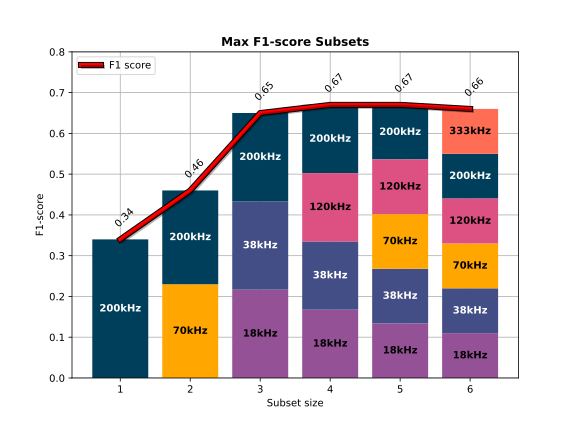
\includegraphics[scale=0.7]{figures/increasing_freq_f1.png}
            \caption[Best frequency combination - F1-score]{Colored blocks indicate the frequency or frequencies resulting in the highest F1-score in each tier of combinations.}
          	\medskip 
            \label{increasing_freq_f1_score_fig}
        \end{figure}

        In figure \ref{increasing_freq_f1_score_fig} the best frequencies combinations based on precision is visualized. The trend is similar to the one based on F1-score, but with the \textit{70kHz} beating the \textit{120kHz} when 4 is used. 
        % Precision
        \begin{figure}[H]
            \centering
            \includegraphics[scale=0.7]{figures/increasing_freq_precision.png}
            \caption[Best frequency combination - Precision]{Colored blocks indicate the frequency or frequencies resulting in the highest precision in each tier of combinations.}
          	\medskip 
            \label{increasing_freq_precision_score_fig}
        \end{figure}
        
        In figure \ref{increasing_freq_recall_score_fig} the best frequencies combinations based on precision is visualized. Here, \textit{70kHz} beats \textit{200kHz} when only one frequency can be used. Further, the steep increase in performance happens already at two frequencies. Indicating that the best combination at this stage already finds most of the \textit{sandeel} class.
        %\clearpage
        \begin{figure}[H]
            \centering
            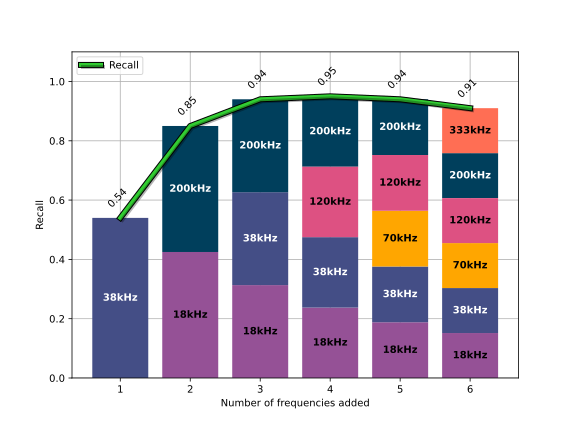
\includegraphics[scale=0.7]{figures/increasing_freq_recall.png}
            \caption[Best frequency combination - Recall]{Colored blocks indicate the frequency or frequencies resulting in the highest recall in each tier of combinations.}
          	\medskip 
            \label{increasing_freq_recall_score_fig}
        \end{figure}

    \subsection{Error bar}
        Figure \ref{errorbar_fig} illustrate a complete plot of all error bars, with sections for each test. The plot has no compltete overview over what frequencies belong to what result, but only a red circle encompassing the error bar related to the combination \textit{18},\textit{38} and \textit{200kHz}. This combination outclasses all other combinations on the same and previous tests, as well as competes with all the results later achieved. In the leftmost section, the red error bar of the 200kHz can be observed as the clear winner. In all other sections, no combinations stands out as the unique regarding F1-score.
        
        \begin{figure}[H]
            \centering
            \includegraphics[scale=0.7]{figures/error_bar.png}
            \caption[Error bar - combinations of 3 frequencies]{Each colored error bar is a combination, and its y-value is the mean F1-score. The error bar's top value is the max value achieved, and the bottom is the lowest. A red circle encompasses the test containing only 18, 38 and 200 kHz. Blue vertical lines sections the error bars into groups where the number of frequencies in each are equal.}
          	\medskip 
            \label{errorbar_fig}
        \end{figure}
        
        
        
    \subsection{Performance trend per frequency}
        Figure \ref{performance_trend_fig} illustrates the performance trend of each frequency. From right to left, the plot shows to that \textit{18kHz}, \textit{38khZ} and \textit{200kHz} all are part of many combinations with high F1-scores. The rest quickly fall in performance, most likely due to not being paired with any of the three previously mentioned. Looking further to the left, \textit{18kHz} seems to have participated in many combinations on average, resulting in high F1-scores. Followed closely by \textit{200kHz}. \textit{333kHz} seems to make the model perform worse by a tiny fraction.
        \begin{figure}[H]
            \centering
            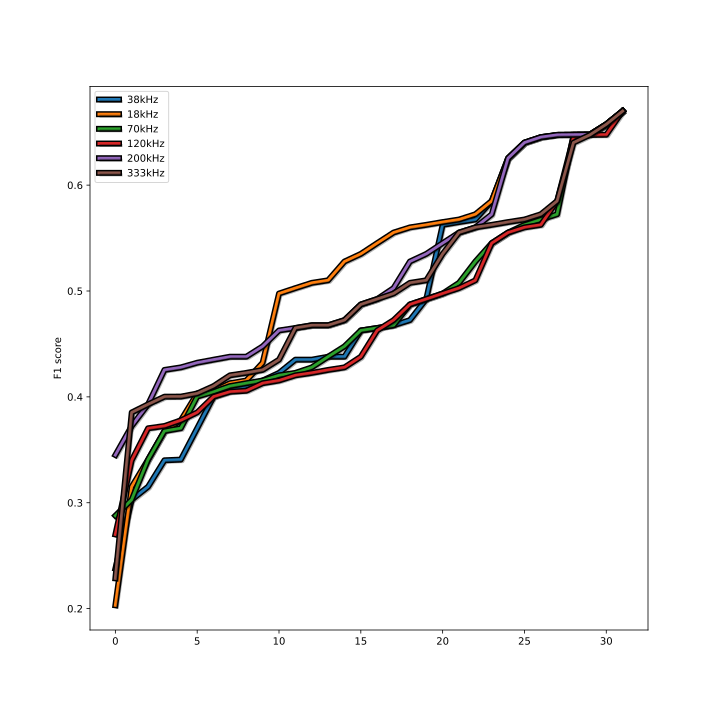
\includegraphics[scale=0.7]{figures/perfomance_trend.png}
            \caption[Performance trend per frequency]{For all combinations containing a certain frequency, the performance is plotted increasingly.}
          	\medskip 
            \label{performance_trend_fig}
        \end{figure}
    
    % Ta det med i diskusjonen?
    A major observation from the results is the relative quick increase in performance, which then stagnates after the best three frequencies is found. This indicates that the information contained in the other frequencies does not contribute in any large measure to the performance. Some might even have a negative impact on the results, as you can see in figure \ref{increasing_freq_f1_score_fig} when the \textit{333kHz} is added. This is a small by a small margin, and figure \ref{performance_trend_fig} does not illustrate that \textit{333kHz} is worse than any large factor. 
    
    
